\documentclass{standalone}
\begin{document}
	\chapter{Ground Glass Identification Pipeline}
	
	Since the end of 2019, COVID-19 has widely spread all over the world. Up to now the gold standard for the identification of the pathology is the 
	RT-PCR even if it is reported that its sensitivity might not be enough for COVID-19 identifications~\cite{ART:Ai},moreover it is time consuming. Several chest CT scans collected from COVID-19 patients shown bilateral patchy shadows or ground glass opacity (GGO) in the 
	lung~\cite{ART:Ai}~\cite{ART:Wang}, which makes this technique suitable to help dignosis, monitoring the course of the disease and check the recovery of healed patients, since the GGO pattern may change according to the status of the disease.\\
	Austin in Glossary of terms for CT of the lungs~\cite{ART:Austin} define the Ground Glass Opacities as hazy increased attenuation of lung, with 
	preservation of bronchial and vascular margins caused by partial filling of air spaces, interstitial thickening, partial collapse of alveoli, normal 
	expiration, or increased capillary blood volume. This kind of lesion is not exclusive of COVID-19 but can be associated to many other pathologies 
	but the study of its particular pattern in combination with other techniques may help early diagnosis of this pathology and the monitoring of the 
	recovery, has shown by ~\cite{ART:Bernheim}.\\
	
	So the identification and quantification of this kind of lesions is very important to help diagnosis, monitor the recovery and understand infection 
	pathogenesis. Up to know the identification of these lesions is made by manual or semi-automatic segmentations, both of them are time consuming, 
	error prone and subjective, since require the interaction of specialized operators. To overcome this issues an automatic way to obtain these information is desiderable, since allows to obtain measures that do not depend n operator subjectivity; moreover it is desiderable to obtain segmentation results in a small amount of time, which is not compatible with manual or semi-automatic segmentation.\\
	
	In this chapter I will describe in details the implementation of a segmentation pipeline which allows a fast and automatic segmentation of GGO. 
	
		 
	
	\begin{figure}\label{fig:HealthVSCovid}
		\centering
		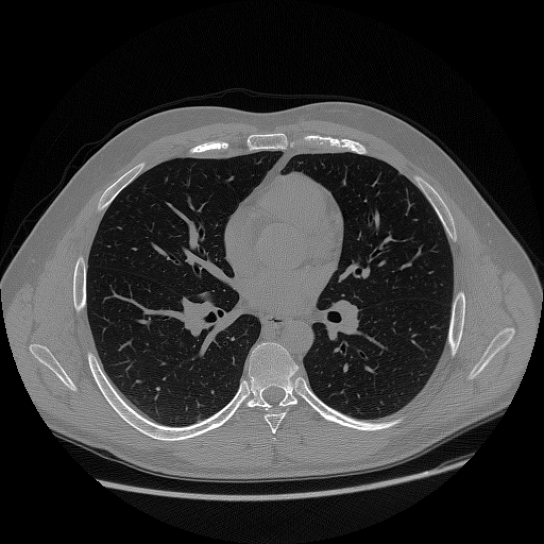
\includegraphics[scale=.5]{healthy.png}
		\quad
		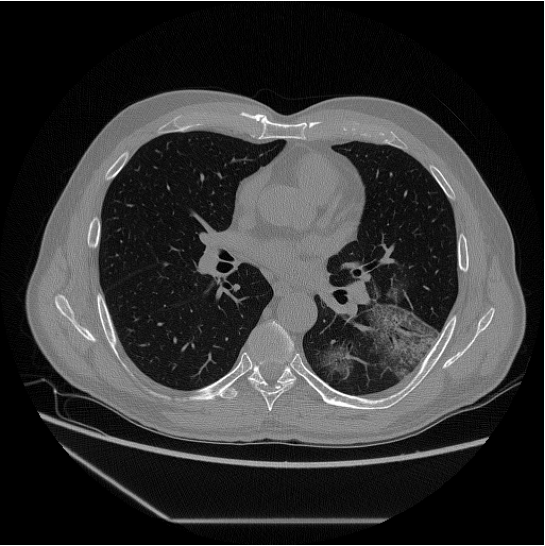
\includegraphics[scale=.5]{ggo.png}
		\caption{CT scan of torax for an healthy patient(left) and a COVID-19 affected one(right) in which we can observe a huge amount of GGO in the right lung}
	\end{figure} 
	
	
\end{document}